\documentclass{tufte-handout}

\title{Föreläsning 1: Permutationer och kombinationer $\cdot$ 1MA020}

\author[Vilhelm Agdur]{Vilhelm Agdur\thanks{\href{mailto:vilhelm.agdur@math.uu.se}{\nolinkurl{vilhelm.agdur@math.uu.se}}}}

%\date{15 januari 2023}


%\geometry{showframe} % display margins for debugging page layout

\usepackage{graphicx} % allow embedded images
  \setkeys{Gin}{width=\linewidth,totalheight=\textheight,keepaspectratio}
  \graphicspath{{graphics/}} % set of paths to search for images
\usepackage{amsmath}  % extended mathematics
\usepackage{booktabs} % book-quality tables
\usepackage{units}    % non-stacked fractions and better unit spacing
\usepackage{multicol} % multiple column layout facilities
\usepackage{lipsum}   % filler text
\usepackage{fancyvrb} % extended verbatim environments
  \fvset{fontsize=\normalsize}% default font size for fancy-verbatim environments

\usepackage{color,soul} % Highlights for text

% Standardize command font styles and environments
\newcommand{\doccmd}[1]{\texttt{\textbackslash#1}}% command name -- adds backslash automatically
\newcommand{\docopt}[1]{\ensuremath{\langle}\textrm{\textit{#1}}\ensuremath{\rangle}}% optional command argument
\newcommand{\docarg}[1]{\textrm{\textit{#1}}}% (required) command argument
\newcommand{\docenv}[1]{\textsf{#1}}% environment name
\newcommand{\docpkg}[1]{\texttt{#1}}% package name
\newcommand{\doccls}[1]{\texttt{#1}}% document class name
\newcommand{\docclsopt}[1]{\texttt{#1}}% document class option name
\newenvironment{docspec}{\begin{quote}\noindent}{\end{quote}}% command specification environment

\include{mathcommands.extratex}

\begin{document}

\maketitle% this prints the handout title, author, and date

\begin{abstract}
\noindent
Vi börjar med att fråga oss vad kombinatorik ens är för något. Sedan introducerar vi några väldigt grundläggande begrepp och principer i ämnet, och tillämpar dem på att diskutera permutationer och kombinationer.
\end{abstract}

\section{Vad är kombinatorik?}

Jag hörde en gång, på en fest under min masterutbildning, en utläggning av en doktorand om att all matematik handlar om att reducera sina problem till en enklare form -- och i slutändan var alla matematikproblem antingen linjär algebra, i vilket fall de var lätta, eller så var de kombinatorik, i vilket fall de var svåra. Vi skall alltså studera den svåra delen av matematiken.

En annan överförenklande kategorisering av matematiken ges oss av Randall Munroe.\cite{XKCD_math_classification} Kombinatorik sysslar med den mellersta sortens problem -- där det är lätt att förstå frågan, och inga märkliga kontinuerliga objekt är involverade, men svaret ändå kan vara komplicerat att ta reda på.

\begin{figure}[h]
	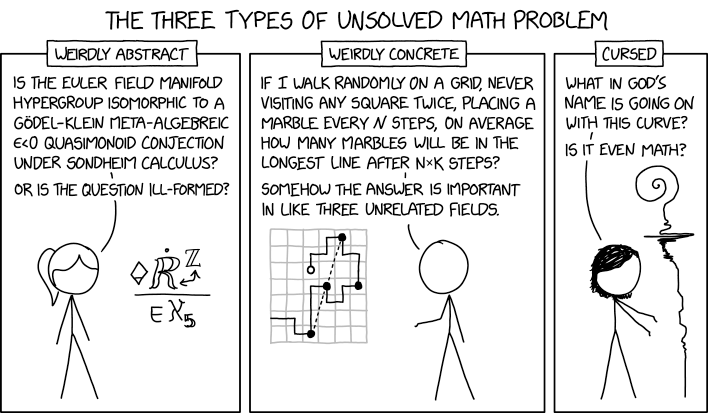
\includegraphics{graphics/unsolved_math_problems.png}
	%\caption{Tre typer av olösta matematikproblem}
\end{figure}

En mer ordboksmässig definition av vad kombinatorik är vore att säga att det handlar om att räkna saker, när sakerna är ändligt många och diskreta. Detta är dock heller ingen precis eller uttömmande definition, så det finns saker som är kombinatorik utan att nödvändigtvis handla om att räkna saker, till exempel inom grafteori.

\section{Varför studera kombinatorik?}

Kombinatorik har som redan nämnts tillämpningar i ren matematik -- många problem inom andra grenar av matematiken kan reduceras till problem i kombinatorik. Det har också otaliga tillämpningar utanför den rena matematiken:
\begin{enumerate}
	\item Nätverk och grafer
	\item Analys av algoritmer
	\item Design av kretskort
	\item Design av experiment
\end{enumerate}
Merparten av alla pussel-spel av typen sudoku, eller ``flytta bilarna för att få ut en specifik bil'', etc., kan ses som rena kombinatorikproblem.

\section{Additions- och multiplikations-reglerna}

\begin{definition}[Additions-regeln]
	Om $A$ är en mängd av $n$ objekt och $B$ är en mängd av $m$ objekt så finns det $n+m$ sätt att välja ett objekt från $A$ \emph{eller} ett objekt från $B$. Eller formulerat i symboler, om $\abs{A} = n$ och $\abs{B} = m$ så är $\abs{A \coprod B} = n + m$.\sidenote{Symbolen $\coprod$ betyder \emph{disjunkt union} -- vi tar unionen av de två mängderna, men vi tvingar mängderna att vara disjunkta genom att komma ihåg vilken mängd varje element kom från.  Så om $A$ och $B$ inte har några gemensamma element är det samma sak som $\cup$, men om de har gemensamma element gäller att t.ex. $\{1,2,3\}\cup \{3,4\} = \{1,2,3,4\}$, emedan $\{1,2,3\} \coprod \{3,4\} = \{(1,A), (2,A), (3,A), (3,B), (4, B)\}$, så de har alltså olika antal medlemmar.

För det allra mesta behöver man inte vara så här rigorös, men det kan vara bra att ha i bakhuvudet att summa-regeln inte räknar antalet element i $A\cup B$ om $A$ och $B$ kan tänkas ha gemensamma element. Vad vi gör i det fallet kommer vi återkomma till senare, när vi diskuterar inklusion-exklusion.}
\end{definition}

\begin{example}\label{example_addition_rule}
En restaurang har en meny med fyra drinkar, fem förrätter, tio huvudrätter, och tre desserter. Hur många saker har de på menyn?

Additions-regeln säger oss att svaret är $4+5+10+3 = 22$.
\end{example}

\begin{definition}[Multiplikations-regeln]
	Om $A$ är en mängd av $n$ objekt och $B$ är en mängd av $m$ objekt så finns det $nm$ sätt att välja ett objekt från $A$ \emph{och} ett objekt från $B$. Eller ekvivalent, det finns $nm$ sätt att välja ett par av ett objekt ur $A$ och ett objekt ur $B$. Eller uttryckt i symboler
$$\abs{A\times B} = \abs{\{(a,b) \given a \in A, b \in B\}} = nm.$$
\end{definition}

\begin{example}
	Om du besöker restaurangen i Exempel \ref{example_addition_rule}, hur många olika sätt finns det att beställa en trerätters middag med en drink till?
\sidenote{En fullständigt teoretisk fråga, eftersom ingen faktiskt har råd med det i dagens ekonomi.} Multiplikations-regeln säger oss att svaret är $4\times 5\times 10\times 3 = 600$.
\end{example}

\section{Strängar}

\begin{definition}
En \emph{sträng} $s$ (eller ett \emph{ord}) av längd $n$ på en mängd $X$ (kallad \emph{alfabetet} för strängen) är en funktion
$$s: \{1, 2, \ldots, n\} = [n] \to X$$
där $s_i$ är den $i$te bokstaven i ordet.\sidenote{Från och med nu kommer vi konsekvent använda notationen $[n]$ för mängden av tal mellan $1$ och $n$.}
Vi skriver detta oftast som $s = x_1x_2\ldots x_n$, där $x_i = s(i)$.
\end{definition}

\begin{example}[Binära strängar]
Låt $X = \{0,1\}$. Strängar $s: [n] \to X$ kallas för \emph{binära strängar}. Det finns $2^n$ strängar av längd $n$.\sidenote{Så det finns till exempel åtta binära strängar av längd tre, nämligen
$$000, 001, 010, 011, 100, 101, 110, 111.$$}

Hur vet vi detta? Det finns två val för varje bokstav, så multiplikationsregeln säger oss att det måste finnas $2\times 2\times\ldots\times 2 = 2^n$ att göra ett val av vad varje bokstav skall vara.
\end{example}

\begin{example}[$m$-ära strängar]
Låt $X = \{0,1,\ldots,m-1\}$. Strängar med detta alfabetet kallas för $m$-ära strängar. Om $m = 2$ är de binära, om $m = 3$ är de ternära. 
\end{example}

För generella $X$ kallar vi en sträng $s: [n] \to X$ för en $X$-sträng.

\section{Permutationer}

\begin{definition}
En sträng $s: [k] \to X$ kallas för en \emph{permutation} av längd $k$ av elementen i $X$ om alla bokstäverna i $s$ är olika, det vill säga om $s(i) \neq s(j)$ ifall $i \neq j$.
\end{definition}

Självklart måste $\abs{X} \geq k$ för att det skall existera några permutationer av längd $k$ av $X$.\sidenote{Hur hade du bevisat det?}

\begin{example}
Låt $X = [3]$. Det finns $6$ permutationer av längd $2$ av $X$\sidenote{Dessa är, specifikt, $$12, 13, 21, 23, 31, 32.$$} -- vi kan se detta med hjälp av multiplikationsprincipen: Vi har tre val av första bokstav, men när vi valt den har vi bara två val kvar av andra bokstav, eftersom vi inte får ha två av samma. Alltså är det totala antalet $3\times 2 = 6$.
\end{example}

\begin{definition}
För $n = 1, 2,\ldots$, definiera $n! = n\times(n-1)\times\ldots\times2\times1$. Definiera $0! = 1$.\sidenote{Att vi låter $0!$ vara lika med ett är för att vi ser det som produkten av inga tal alls, vilket är bekvämt att se som att det blir $1$. Varför detta är så kommer vi kanske att återkomma till när vi pratar om rekursioner.}

För $k \leq n$, definiera $P(n,k) = \frac{n!}{(n-k)!}$. Lägg märke till att $P(n,n) = \frac{n!}{(n-n)!} = \frac{n!}{0!} = n!$.
\end{definition}

\begin{proposition}
Om $\abs{X}=n$ och $0 \leq k \leq n$ så finns det $P(n,k)$ permutationer av längd $k$ från $X$.
\begin{proof}
Vi bevisar detta med hjälp av multiplikationsprincipen -- så vi skall räkna hur många sätt vi kan välja vår permutation $x_1x_2\ldots x_k$ på. Det finns så klart $\abs{X} = n$ sätt att välja första bokstaven $x_1$ i vår permutation. När vi sedan skall välja $x_2$ får den inte vara lika med $x_1$, så vi väljer ett element ur $X \setminus \{x_1\}$, och $\abs{X\setminus\{x_1\}} = n-1$. Likaledes för $x_3$ så får den varken vara lika med $x_1$ eller $x_2$, så vi väljer från $X\setminus \{x_1, x_2\}$, och har $n-2$ val.

Den här processen fortsätter tills vi skall välja $x_k$, och i det skedet har vi tagit bort $k-1$ val, och har alltså $\abs{X \setminus \{x_1, x_2, \ldots, x_{k-1}\}} = n - (k-1)$ val.

Multiplikationsregeln säger oss att det totala antalet permutationer är lika med produkten av antalet val vi hade i varje steg, det vill säga
\begin{align*}
	n\cdot(n-1)\cdot(n-2)\cdot\ldots\cdot(n-(k-1)) &= \frac{n\cdot(n-1)\cdot(n-2)\cdot\ldots\cdot2\cdot1}{(n-k)\cdot\ldots\cdot2\cdot1}\\
	&= \frac{n!}{(n-k)!} = P(n,k).
\end{align*}
\end{proof}
\end{proposition}

\begin{example}
	På hur många olika sätt kan $n$ personer sitta runt ett runt bord?\sidenote{Det finns en liten ritning av detta i anteckningarna från föregående år, och jag lär rita den på den faktiska föreläsningen.}

	Det finns två olika sätt vi kan se på frågan\sidenote{Detta är ett exempel av skillnaden mellan problem med etiketter och utan, vilket är ett generellt fenomen som kommer återkomma gång på gång. Här är det platserna runt bordet som kan ha etiketter eller inte. Var noggrann med att fundera kring vilken typ av } -- antingen är det skillnad på de olika stolarna runt bordet (vissa kan se ut genom fönstret, andra inte), så att vi får olika sätt att placera folk runt bordet genom att rotera hela placeringen, eller så är det enda som spelar roll ordningen de sitter i, och vi ser olika rotationer av samma ordning som samma sätt att sitta runt bordet.

	Om platserna har etiketter, så att det inte bara är ordningen som spelar roll, så kan vi numrera platserna från plats $1$ till plats $n$. Om vi kallar mängden med gäster för $X$ blir alltså varje placering ett $X$-ord -- vi kan skriva den som ``gäst ett, gäst två, etc.''. Och eftersom varje person bara kan sitta på en stol blir detta alltså en permutation -- och vi vet att det finns $n!$ permutationer av längd $n$ ur ett alfabete med $n$ bokstäver.

	Om platserna är oetiketterade, det vill säga att det enda vi bryr oss om är ordningen folk sitter i, får vi räkna på ett annat sätt. Givet en placering kan vi godtyckligt välja en person som ``först'', och sedan numrera platserna i medurs ordning. För varje av de $n$ sätten att välja vem som är först får vi alltså en placering där platserna har etiketter.

	Detta ger oss ett annat sätt att räkna antalet placeringar med etiketter -- vi räknar antalet utan etiketter, kallar det $m$, och får alltså att antalet med etiketter är $nm$.

	Men eftersom vi redan vet att antalet när platserna har etiketter är $n!$ så får vi alltså av detta att $n! = nm$, eller $m = \frac{n!}{n} = (n-1)!$.\sidenote{Detta är ett vanligt sätt att resonera inom kombinatorik -- vi hittade två olika sätt att räkna samma sak, och fick på så sätt ut en likhet ($nm = n!$) som vi kunde använda för att räkna en annan sak.}
\end{example}

\section{Kombinationer}

Detta avsnitt kommer skrivas snart.

\bibliography{references}
\bibliographystyle{plainnat}



\end{document}
